\section{Konzeption}

Nachfolgend soll nun zunächst die aktuelle Produktiv- und die aktuellen Testumgebungen der Pixelhouse GmbH beschrieben werden. Dabei werden diese in Bezug auf typische Schwächen beziehgunsweise Probleme von Systemumgebungen untersucht. Anschließend soll ein Konzept für eine neue Testumgebung beschrieben werden, das mit Hilfe der im Kapitel Grundlagen erarbeiteten Kenntnisse zur Virtualisierung die zuvor beschriebenen Probleme umgeht. Es wird außerdem eine Auswahl zweier konkreter Virtualisierungstechnologien getroffen, mit deren Hilfe später eine Implementierung des Konzepts erfolgt.

\subsection{Beschreibung der aktuellen Produktivumgebung}

Die Betriebsumgebung, die von der Pixelhouse GmbH in Produktion eingesetzt wird, besteht aus einer Vielzahl von Komponenten und Diensten. Diese Komponenten werden bislang jeweils auf echter Serverhardware betrieben.

\begin{figure}[!ht]
  \begin{center}
    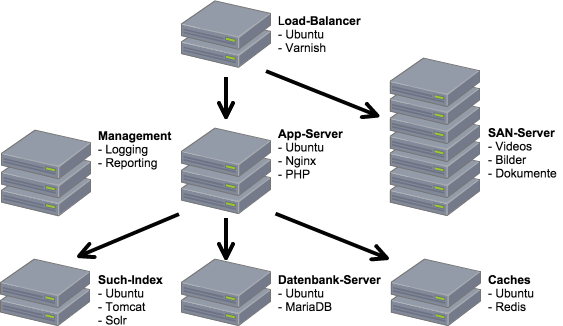
\includegraphics[width=14cm]{bilder/Produktiv-Umgebung.png}
    \caption{Die Produktivumgebung der Webseite Chefkoch.de}
    \label{produktion}
  \end{center}
\end{figure}

Der Aufbau der Produktivumgebung ist in der Abbildung \ref{produktion} zu sehen. Im Zentrum der Infrastruktur stehen insgesamt drei Appserver. Bei jedem Appserver handelt es sich dabei um einen Ubuntu-Server, auf dem der Webserver Nginx \citep{nginx:001} und der Script-Interpreter \ac{PHP} \citep{php:001} ausgeführt wird, um HTTP-Anfragen mit Hilfe statischer oder dynamische Inhalte zu beantworten. Auf den App-Servern läuft somit auch die in \ac{PHP} geschriebene Anwendung selbst. Für die langfristige Datenhaltung greifen die PHP-Scripte dabei auf zwei Datenbankserver (Master und Slave) zu, auf denen ebenfalls Ubuntu und der Mysql-Fork MariaDB \citep{mariadb:001} installiert sind. Für kurzfristige und hochverfügbare Datencaches gibt es zwei Ubuntu-Server (Master und Slave) auf denen der Key-Value-Store Redis \citep{redis:001} läuft. Zudem wird auf weiteren zwei Ubuntu-Servern (Master und Slave) ein Such-Index mit Hilfe der Suchmaschine Solr \citep{solr:001} betrieben, die als Java-Anwendung in einem Tomcat-Application-Server \citep{tomcat:001} läuft. Binärdateien (Videos, Bilder, Dokumente, etc.) werden auf insgesamt 7 weiteren Servern redundant abgelegt. Damit die Appserver und die SAN-Server (\acl{SAN}) von außen unter einheitlichen HTTP-Adressen erreichbar sind und sich die Last gleichmäßig auf die einzelnen Server verteilt, landen sämtliche HTTP-Anfragen per DNS-Round-Robin zunächst bei einem von zwei Ubuntu-Servern, auf denen Varnish \citep{varnish:001} als Load-Balancer installiert ist. Diese nehmen die Anfragen entgegen und verteilen sie an die dahinter liegenden Server. Varnish ist zudem ein effizienter HTTP-Cache, der in der Lage ist, die von den App- oder SAN-Servern zurückgelieferten Antworten zu cachen und bei erneuter Anfrage selbst auszuliefern. Zu guter Letzt gibt es noch drei weitere Server, auf denen Software für die Administration und das Reporting läuft.

Das größte Problem der aktuellen Produktivumgebung ist, dass sie manuell konfiguriert wird. Änderungen an der Konfiguration werden typischerweise in einer Nachtschicht durchgeführt und anschließend händisch getestet. Dies hat in der Vergangenheit schon mehrfach zu Ausfällen geführt. Humble und Farley beschreiben in ihrem Buch eine sinnvolle Alternative: "`The change you want to make shold first have been tested on one of your production like testing environments, and automated tests should be run to ensure that it doesn't break any of the applications that use the environment. The change should be made to version control and then applied through your automated process for deploying infrastructural changes."' \citep[S.][S. 287]{HumFar10} Die aktuellen Testumgebungen, die nun im nächsten Unterkapitel beschrieben werden, ähneln der Produktion bisher aber nur wenig.

\subsection{Beschreibung der aktuellen Testumgebungen}

Die aktuellen Testumgebungen der Pixelhouse GmbH besitzen einen extrem reduzierten Aufbau. Dieser wird in Abbildung \ref{alte-test} gezeigt. Die Testumgebungen werden alle auf ein und derselben Hardware-Maschine installiert. Fast alle Komponenten der zuvor beschriebenen Produktivumgebung werden dabei von den einzelnen Testumgebungen gemeinsam verwendet. Beispielsweise nutzen alle Testumgebungen den gleichen Varnish für das Load-Balancing und Caching. Dieser reicht die HTTP-Anfragen an den selben Nginx-Web-Server und PHP-Interpreter weiter und puffert die Antworten bei Bedarf gleichermaßen. Als Backend-Dienste werden dieselbe MariaDB-Datenbank, derselbe Redis-Cache und derselbe Solr-Such-Index verwendet. Die Binärdateien werden ebenfalls auf demselben Host von allen Testumgebungen gemeinsam verwendet. Einziger Unterschied zwischen den einzelnen Testumgebungen ist, dass aufgrund einer speziellen Konfiguration im Nginx-Webserver je nach aufgerufener URL (\acl{URL}) vom PHP-Interpreter andere PHP-Scripte geladen werden und somit jeweils eine andere Version der PHP-Anwendung getestet werden kann.

\begin{figure}[!ht]
  \begin{center}
    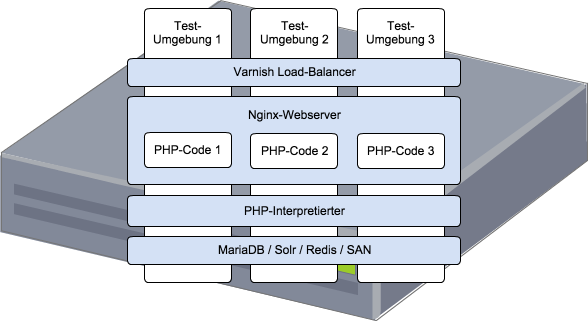
\includegraphics[width=14cm]{bilder/Aktuelle-Testumgebung.png}
    \caption{Die aktuelle Testumgebung}
    \label{alte-test}
  \end{center}
\end{figure}

Wegen der Unterschiede zur Produktivumgebung eignen sich die Testumgebungen grundsätzlich nicht zum aussagekräftigen Testen von Infrastrukturänderungen. Hinzu kommt, dass Änderungen an den gemeinsam genutzten Komponenten immer alle Testumgebungen gleichermaßen betreffen. Dies kann zum Beispiel dazu führen, dass ein Produktmanager beim Testen eines neuen Features Fehler sieht, obwohl diese nicht durch das neue Feature sondern eben durch die Änderungen an der Infrastruktur ausgelöst wurden.

Ein weiteres Problem der aktuellen Testumgebungen ist, dass sie sich die Testdaten teilen. Dies ist immer dann problematisch, wenn es sich um einen schreibenden Datenzugriff handelt. So ist es zum Beispiel nicht möglich, dass zwei Tests versuchen, sich mit der gleichen E-Mail-Adresse zu registrieren. Humble und Farley empfehlen für Testumgebung deshalb allgemein die sogenannte Test Isolation \citep[Vgl.][S. 337]{HumFar10}. Dabei handelt es sich um eine Strategie, die jeden Test von anderen Tests in Bezug auf seine Daten unabhängig macht. Eine mögliche Implementierung einer solchen Strategie wäre es zum Beispiel, das Transaktionssystem der Datenbank auszunutzen, damit verschiedene Datenbank-Verbindungen sich nicht gegenseitig beeinflussen. Eine weitere Möglichkeit wäre, die Daten innerhalb der Datenbank zu partitionieren, indem man die Entitäten in der Datenbank zum Beispiel aufgrund einer Namenskonvention bestimmten Tests zuordnet. Da das Datenbankschema der Seite Chefkoch.de über einige Jahre historisch gewachsen ist und an vielen Stellen ohne explizite Datenbank-Constraints (wie zum Beispiel Foreign-Keys) definiert wurde, sind alle Versuche, innerhalb der Datenbank eine Isolation der Testdaten zu erreichen, bisher gescheitert.

Im Folgenden soll nun eine neue Testumgebung auf Basis von Virtualisierung konzipiert werden, in der diese Probleme nicht mehr auftreten können.

\subsection{Definition einer neuen Testumgebung}

\begin{figure}[!ht]
  \begin{center}
    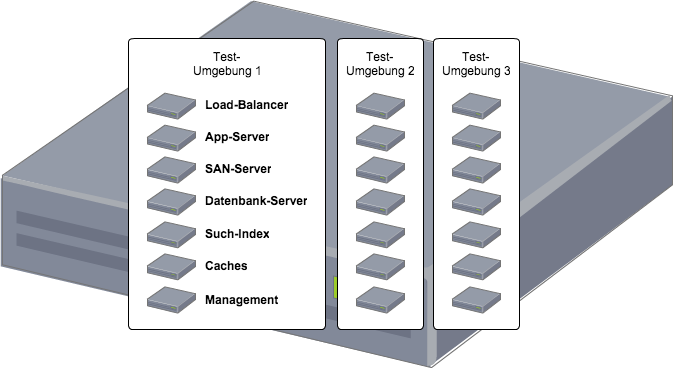
\includegraphics[width=14cm]{bilder/Untersuchungs-Umgebung.png}
    \caption{Definition der neuen Testumgebungen}
    \label{neue-test}
  \end{center}
\end{figure}


Wie im Kapitel Grundlagen beschrieben, gibt es eine Reihe von Technologien, mit denen man auf einer Hardware-Maschine mehrere künstliche Maschinen simulieren kann. Es ist also zum Beispiel möglich, auf ein und der selben Hardware-Maschine mehrere Datenbankserver nebeneinander laufen zu lassen. Statt also zum Beispiel mit Hilfe von Transaktionen oder einer Partitionierung eine Isolation innerhalb der Datenbank zu erreichen, bekommt jede Testumgebung einen komplett eigenen Datenbankserver zugewiesen. Es kann somit nicht vorkommen, dass ein Test in der einen Testumgebung die Daten eines Testes in einer anderen Testumgebung direkt verändert.

Zudem ist es grundsätzlich sogar möglich, alle Komponenten der Produktivumgebung für jede Testumgebung neu zur Verfügung zu stellen. In der Theorie kann also jede Testumgebung genau den gleichen Aufbau wie die Produktivumgebung besitzen. Bei der Implementierung werden wir prototypisch alle Komponenten bis auf den Management- und SAN-Server erzeugen, da diese für die eigentliche Anwendung der Seite Chefkoch.de keine Rolle spielen.

Solange die konkrete Virtualisierungslösung außerdem die Möglichkeit bietet, die Zustände der einzelnen Maschinen zu sichern, ist es möglich, Konfigurationsänderungen an den Komponenten nachzuhalten und in unterschiedlichen Testumgebungen mit verschiedenen Versionsständen der Konfiguration zu arbeiten. 

Der Aufbau der angestrebten Testumgebung ist noch einmal in der Abbildung \ref{neue-test} zu sehen.

\subsection{Verwendete Virtualisierungslösungen}

Im Folgenden Hauptkapitel sollen nun zwei konkrete Lösungen zur Erzeugung von Testumgebungen implementiert werden. Die konkret verwendeten Virtualisierungslösungen werden dabei von der Pixelhouse GmbH vorgegeben: Oracle VirtualBox und Docker.

Zum einen setzt die Pixelhouse GmbH bereits Oracles VirtualBox ein, um eine lokale Entwicklungsumgebung für die Anwendung der Webseite Chefkoch.de auf den Laptops der Entwickler vorzuhalten. VirtualBox ist somit bereits auf fast allen Rechnern vorhanden und es existieren grundlegende Kenntnisse und Erfahrungen für dieses Produkt.

Zum anderen wird aktuell von Seiten der Server-Administratoren das Produkt Docker eingeführt, um damit Teile der Produktivumgebung der Plattform zu betreiben. Erste Produktiv-Komponenten der Webseite Chefkoch.de laufen also bereits innerhalb von Linux-Containern. Die ersten Erfahrungen der Administratoren sind dabei vielversprechend. Es besteht der Wunsch, zukünftig Probleme zu minimieren, die auftreten, weil Entwicklungs-, Test- und Produktivumgebungen nicht die gleiche Technologie verwenden und sich so grundlegend voneinander unterscheiden. Es würde sich also aus Sicht der System-Administratoren anbieten, auch für die Testumgebungen Docker einzusetzen.
